\documentclass[tikz,border=10pt]{standalone}
\usepackage{tikz}
\usetikzlibrary{mindmap}

\begin{document}
\pagestyle{empty}

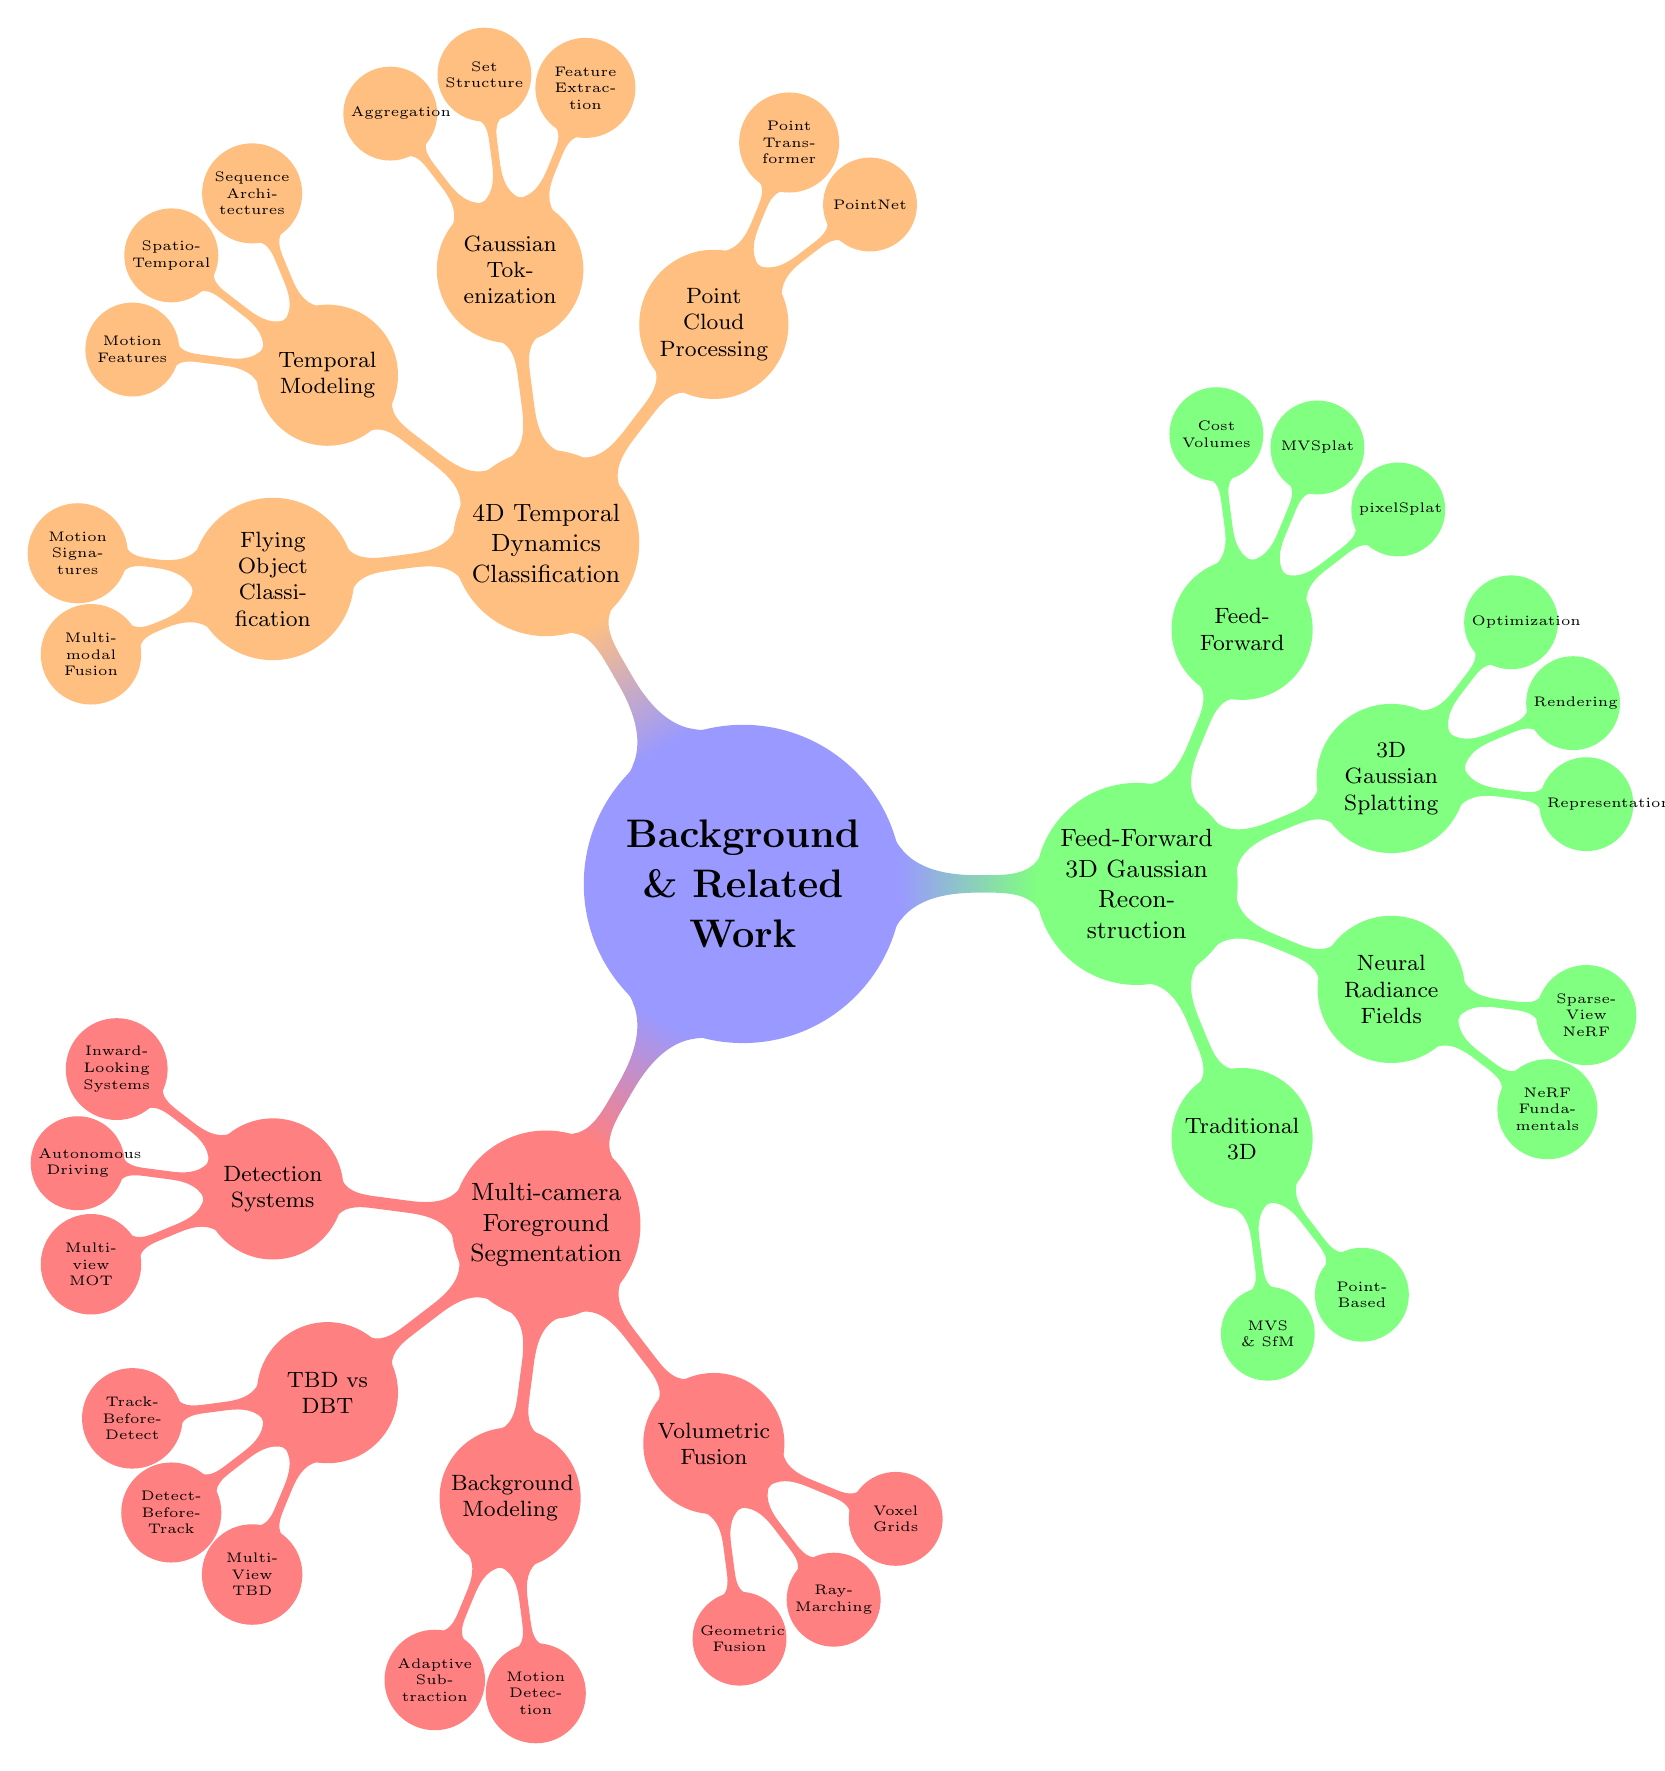
\begin{tikzpicture}[mindmap,
    grow cyclic,
    every node/.style=concept,
    concept color=blue!40,
    level 1/.append style={level distance=5cm,sibling angle=120},
    level 2/.append style={level distance=3.5cm,sibling angle=45},
    level 3/.append style={level distance=2.5cm,sibling angle=30}]

\node[concept, font=\Large\bfseries] {Background \& Related Work}
    child[concept color=red!50] { node {Multi-camera Foreground Segmentation}
        child { node {Detection Systems}
            child { node {Inward-Looking Systems} }
            child { node {Autonomous Driving} }
            child { node {Multi-view MOT} }
        }
        child { node {TBD vs DBT}
            child { node {Track-Before-Detect} }
            child { node {Detect-Before-Track} }
            child { node {Multi-View TBD} }
        }
        child { node {Background Modeling}
            child { node {Adaptive Subtraction} }
            child { node {Motion Detection} }
        }
        child { node {Volumetric Fusion}
            child { node {Geometric Fusion} }
            child { node {Ray-Marching} }
            child { node {Voxel Grids} }
        }
    }
    child[concept color=green!50] { node {Feed-Forward 3D Gaussian Reconstruction}
        child { node {Traditional 3D}
            child { node {MVS \& SfM} }
            child { node {Point-Based} }
        }
        child { node {Neural Radiance Fields}
            child { node {NeRF Fundamentals} }
            child { node {Sparse-View NeRF} }
        }
        child { node {3D Gaussian Splatting}
            child { node {Representation} }
            child { node {Rendering} }
            child { node {Optimization} }
        }
        child { node {Feed-Forward}
            child { node {pixelSplat} }
            child { node {MVSplat} }
            child { node {Cost Volumes} }
        }
    }
    child[concept color=orange!50] { node {4D Temporal Dynamics Classification}
        child { node {Point Cloud Processing}
            child { node {PointNet} }
            child { node {Point Transformer} }
        }
        child { node {Gaussian Tokenization}
            child { node {Feature Extraction} }
            child { node {Set Structure} }
            child { node {Aggregation} }
        }
        child { node {Temporal Modeling}
            child { node {Sequence Architectures} }
            child { node {Spatio-Temporal} }
            child { node {Motion Features} }
        }
        child { node {Flying Object Classification}
            child { node {Motion Signatures} }
            child { node {Multi-modal Fusion} }
        }
    };

\end{tikzpicture}

\end{document}
